\section{Heuristic optimization}

A heuristic is a problem-solving strategy that is based on rules
of thumb or common sense, possibly also using expert
knowledge. Heuristics are often used when no efficient (exact) algorithms
are known, or when applying such algorithms would take too
long.

\subsection{Hill Climbing}
Search for improvements in neighborhood and improve current solution successively.

\begin{enumerate}
    \item Initialization: Start with random solution. \\
    Evaluate initial solution.
    \item Iteratively: \\
    Explore neighborhood and evaluate new solution candidates. Continue with best solution found, if this improves the target function. (Otherwise we’re in a local optimum.)
    \item Return solution
\end{enumerate}

\begin{tcolorbox}[colback=red!5!white,colframe=red!75!black]
Variant: Always take best solution from neighborhood, even if this decreases target function. Pros and cons?
\begin{itemize}
    \item Might escape from local optima.
    \item Not monotone increasing.
    \item Might go back and forth, i.e. run into a cycle.
\end{itemize}
\end{tcolorbox}

\subsubsection{Stochastic hill climbing}

\begin{enumerate}
    \item Initialization: Start with random solution. \\
    Evaluate initial solution.
    \item Iteratively: \\
    Choose random solution in neighborhood (i.e. perform a
random modification). Evaluate new solution candidate,
and accept it, if it is better. Continue until termination
criterion is reached.
    \item Return solution
\end{enumerate}

\clearpage
\subsubsection{Continuous hill climbing}

\begin{enumerate}
    \item Initialization: $i = 0$:
    Initial solution $x_0$.
    \item Iteration $i \rightarrow i + 1$: \\
        $x_{i+1} =
        \begin{cases}
        y_i       & \quad \text{if } f(y_i) \leq f(x_i)\\
        x_i       & \quad \text{if } f(y_i) > f(x_i)
        \end{cases}$
        \item Return solution
\end{enumerate}

\subsection{Tabu search}
Similar to hill climbing, but with some memory. Try to avoid steps that go back to previously visited solutions, or
that undo the effect of previous steps. (These steps are „tabu“.). The goal is to promote diversity of the solutions explored, in
particular to reduce cyclic behaviour and to escape from local
optima.

\begin{enumerate}
    \item Start with random solution. \\
        Evaluate initial solution.
    \item Iteratively: \\
    Explore neighborhood and evaluate new solution
candidates. Only consider steps that are not tabu.
Proceed with step 2 with the best solution found and
update tabu list until termination criterion is reached.
    \item Return solution
\end{enumerate}

\subsubsection{Tabu List}
\begin{itemize}
    \item Simplest variant: Only store last solution as a tabu (to
avoid going back and forth).
\item Probably better: Keep e.g. a tabu list corresponding to last
k moves.
\item How restrictive should the tabus be? (Forbid specific
configurations, whole classes of moves, certain values for
certain variables, ...?)
\item Duration of tabus (short- vs. mid- vs. longterm)?
Size and organization of tabu list(s)?
\item Are the tabus enforced strictly or do we allow exceptions
(„aspiration“)? When and why?
\end{itemize}

\subsubsection{Randomized tabu search}
\textbf{Stochastic version.}

\begin{enumerate}
    \item Start with random solution. \\
        Evaluate initial solution.
    \item Iteratively: \\
Choose a random solution from the neighborhood.
Evaluate the new solution candidate, if its not tabu.
If a better solution is found, continue with this solution,
update tabu list and proceed with step 2. Continue until
termination criterion is reached.
    \item Return solution
\end{enumerate}

\subsection{Simulated annealing}
Similar to hill climbing, but also allow non-improving
moves to escape from local optima.

\begin{enumerate}
    \item Start with random solution. \\
        Evaluate initial solution.
    \item Iteratively: \\
Choose random solution in neighborhood and evaluate it. If
it is better, accept it. If it is worse, accept it only with some
probability.
Continue until termination criterion is reached.
    \item Return solution
\end{enumerate}

With other words

\begin{enumerate}
    \item Initialization: \\
    Start with $x_0$
    \item Iteratively: $x_i \rightarrow x_{i+1}$ \\
    Sample a random solution $y_i$ in the neighborhood and accept it to be $x_{i+1}$ with probability $min\{ 1, e^{\frac{f(x_i)-f(y_i)}{T_i}}\}$
\end{enumerate}

\subsection{Population based methods}
An evolving population of (partial) solutions, whose
members evolve and adapt individually to the problem and are
searching for the optimum. Problem-specific information can be
exchanged between the members of the population, and can
also be passed on to descendants.

\clearpage
\subsection{Genetic Algorithms}

\begin{figure}[H]
\centering
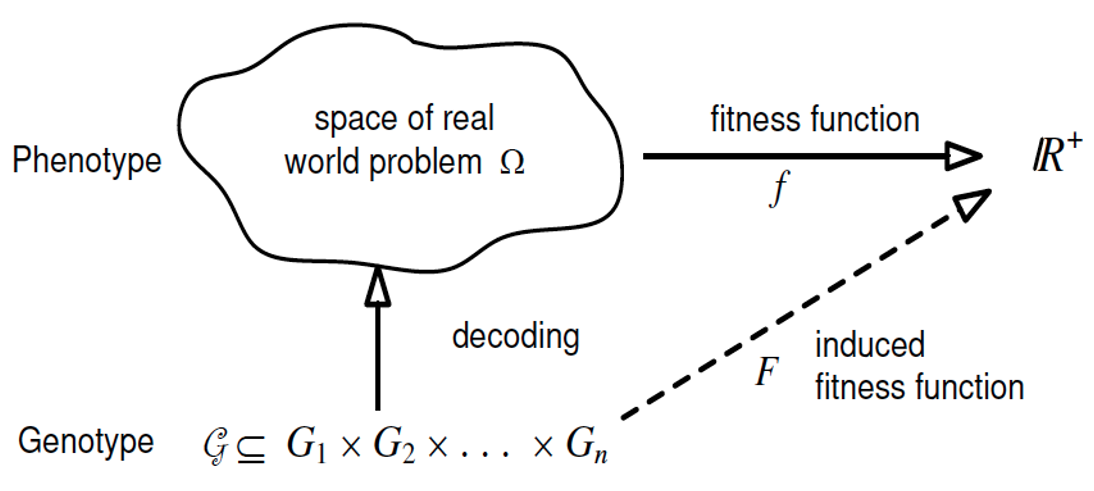
\includegraphics[width=0.6\textwidth]{figures/encodingGenotype.png}
\caption{Genotype encoding}
\end{figure}

\begin{figure}[H]
\centering
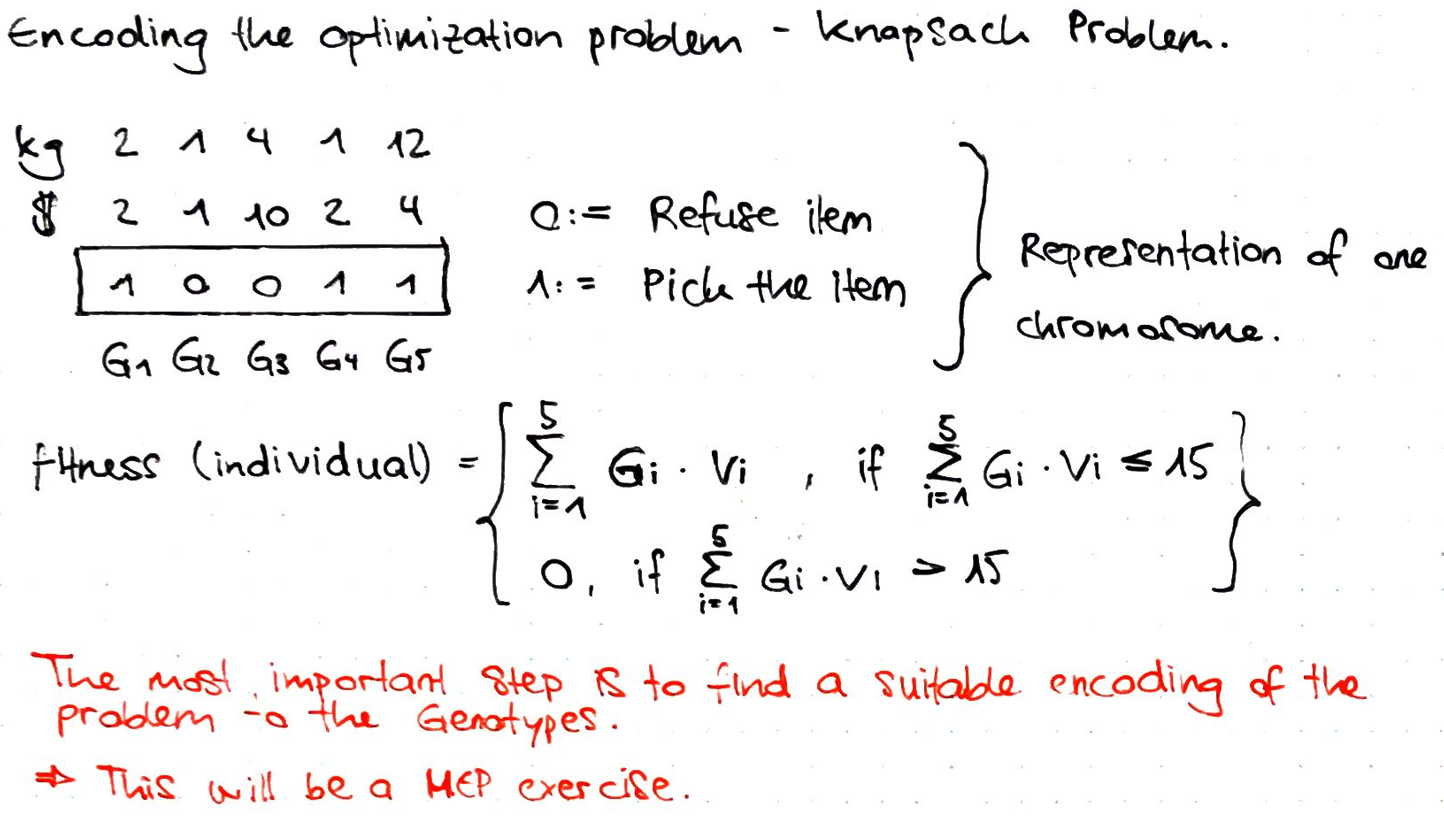
\includegraphics[width=0.9\textwidth]{figures/knapsackGenotype.png}
\caption{Genotype encoding - Knapsack Example}
\end{figure}

A small change in genotype should corresponds to a small
change in phenotype.

Important points in the evolutionary process, i.e. when creating a new generation:
\begin{itemize}
    \item Population development
    \item Natural selection: Selection of individuals for reproduction
    \item Recombination
    \item Mutation
\end{itemize}

\clearpage
\subsubsection{Terminology}

An \textbf{individual} is often represented as a vector with $n$ (binary, integer or
real) entries. The individual entries in (e.g.) the vector representation of an
individual are its \textbf{genes}. They describe the genetic information and the properties of the
individuals. E.g., the individual (0, 0, 1, 0, 1) (binary encoding) consists of
five genes.

The concrete values of a gene can take in an individual are
called \textbf{alleles}. In binary-encoded individuals, the only possible alleles are 0
and 1.

The \textbf{population}is the set of all individuals in an optimization
problem at a given time. A \textbf{generation} is the population at a specific point in time.

The \textbf{genotype} is the encoded form of an individual. The \textbf{phenotype} is the decoded form of an individual. It does
not depend on our choice of encoding. The \textbf{fitness function} is our measure for the quality of a
solution candidate in the optimization problem.

\subsubsection{Algorithm}

\begin{enumerate}
    \item \textbf{Initialization:} Random starting population
    \item \textbf{Iteratively:} Create next generation according to
evoluationary principles: 
\begin{itemize}
    \item Assign fitness to individuals
    \item Natural selection and choosing parents for reproduction
    \item Recombination process
    \item Mutation process
\end{itemize}
Repeat 2 until termination criterion is satisfied
\item Return best individual
\end{enumerate}

\subsubsection{Selection Pressure}
Better individuals should have a higher
chance of reproduction.
\begin{itemize}
    \item \textbf{Better exploration} of search space when selection pressure is \textbf{low}.
    \item \textbf{Better exploitation} of good individuals when selection pressure is \textbf{high}. \\
    Be careful with dominant solution candidates $\rightarrow$ crowding
\end{itemize}

\textbf{Strategy:}Low selection pressure early on, increasing selection
pressure in later generations. (Compare with simulated
annealing.)

\clearpage
\subsubsection{Recombinations}

\textbf{One-Point Crossover}
\begin{figure}[H]
\centering
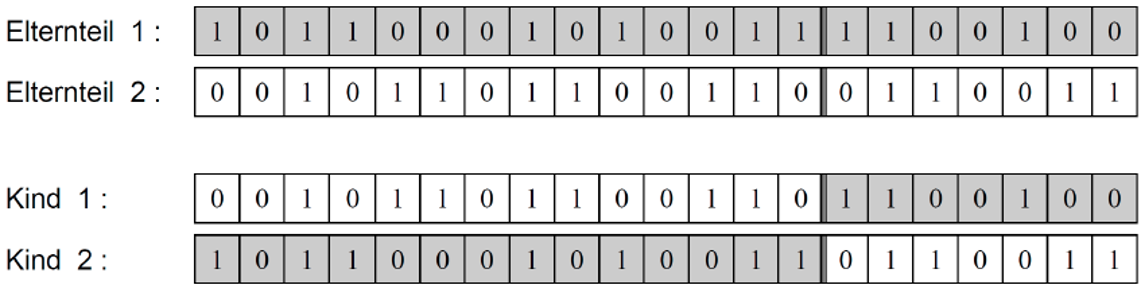
\includegraphics[width=0.5\textwidth]{figures/onepointcrossover.png}
\caption{One-Point Crossover}
\end{figure}

\textbf{Two-Point Crossover}
\begin{figure}[H]
\centering
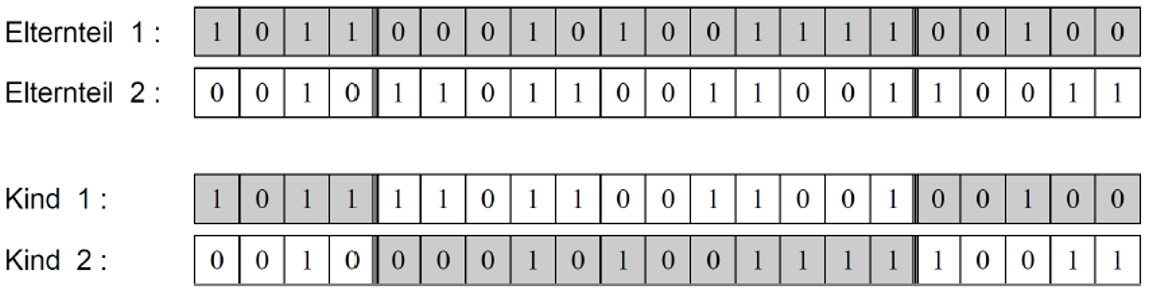
\includegraphics[width=0.5\textwidth]{figures/twopointcrossover.png}
\caption{Two-Point Crossover}
\end{figure}

\textbf{Repair Mechanism for Two-Point Crossover}
\begin{figure}[H]
\centering
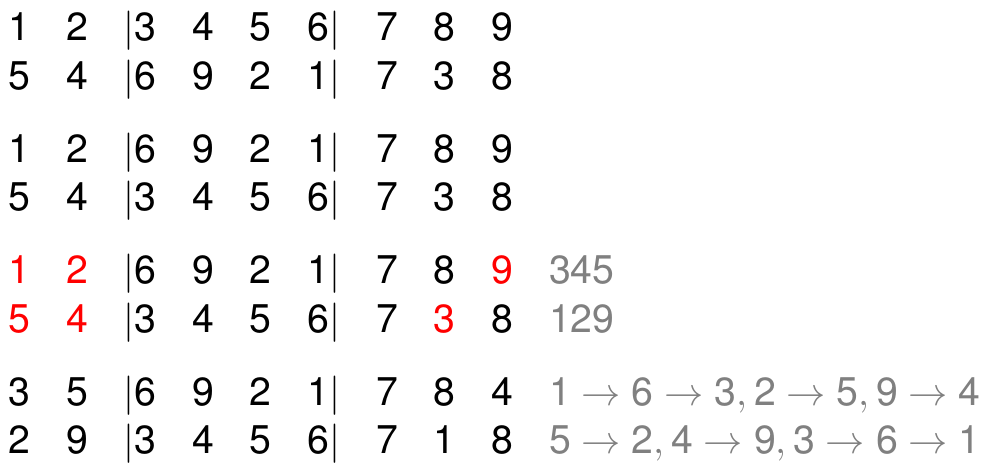
\includegraphics[width=0.4\textwidth]{figures/repairtwopointcrossover.png}
\caption{Repair Mechanism for Two-Point Crossover}
\end{figure}

\textbf{Uniform Crossover}
\begin{figure}[H]
\centering
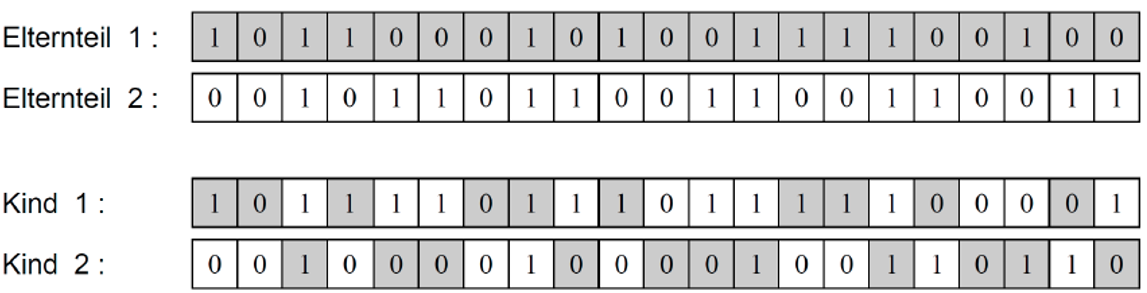
\includegraphics[width=0.5\textwidth]{figures/uniformcrossover.png}
\caption{Uniform Crossover}
\end{figure}

\textbf{Adjacency method}
\begin{figure}[H]
\centering
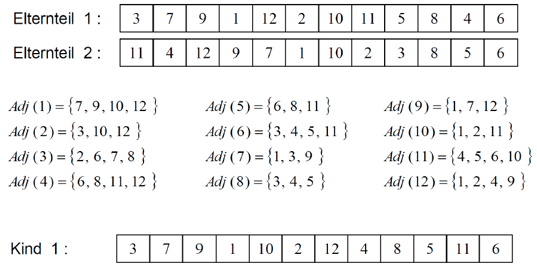
\includegraphics[width=0.5\textwidth]{figures/adjacencyMethod.png}
\caption{Adjacency Method}
\end{figure}

\clearpage
\subsubsection{Mutations}
Important to obtain new solution candidates (diversification) for exploration of search space.

\begin{figure}[H]
\centering
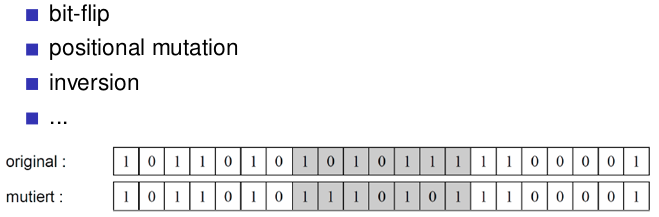
\includegraphics[width=0.6\textwidth]{figures/mutations.png}
\caption{Mutations}
\end{figure}

\subsubsection{Combination}

\begin{figure}[H]
\centering
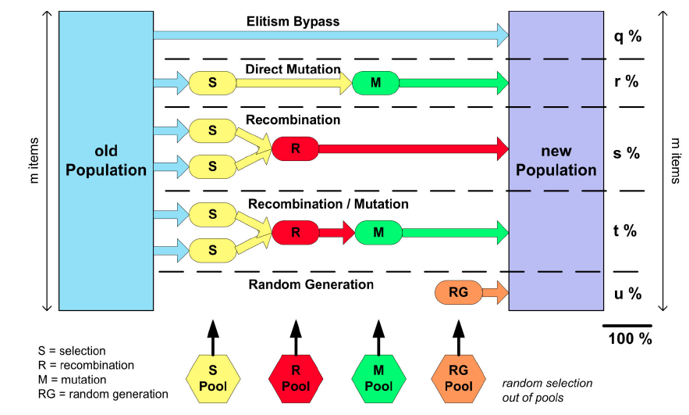
\includegraphics[width=0.9\textwidth]{figures/combination.png}
\caption{Combination}
\end{figure}

\subsection{Ant Colony}
\begin{itemize}
    \item No central instance that coordinates ants. The colony is self-organized. Ants are indpendent from each other. 
    \item An individual ant lays down pheromone trails when looking for food. 
    \item The higher the pheromone concentration on a path, the higher the probability an ant chooses it. If an ant lays down pheromone at a constant rate, shorter paths receive more pheromone per time. $\rightarrow$ Frequently used good paths are reinforced and attract even more ants.
    \item Unused paths become unattractive because of evaporation.
\end{itemize}

\begin{figure}[H]
\centering
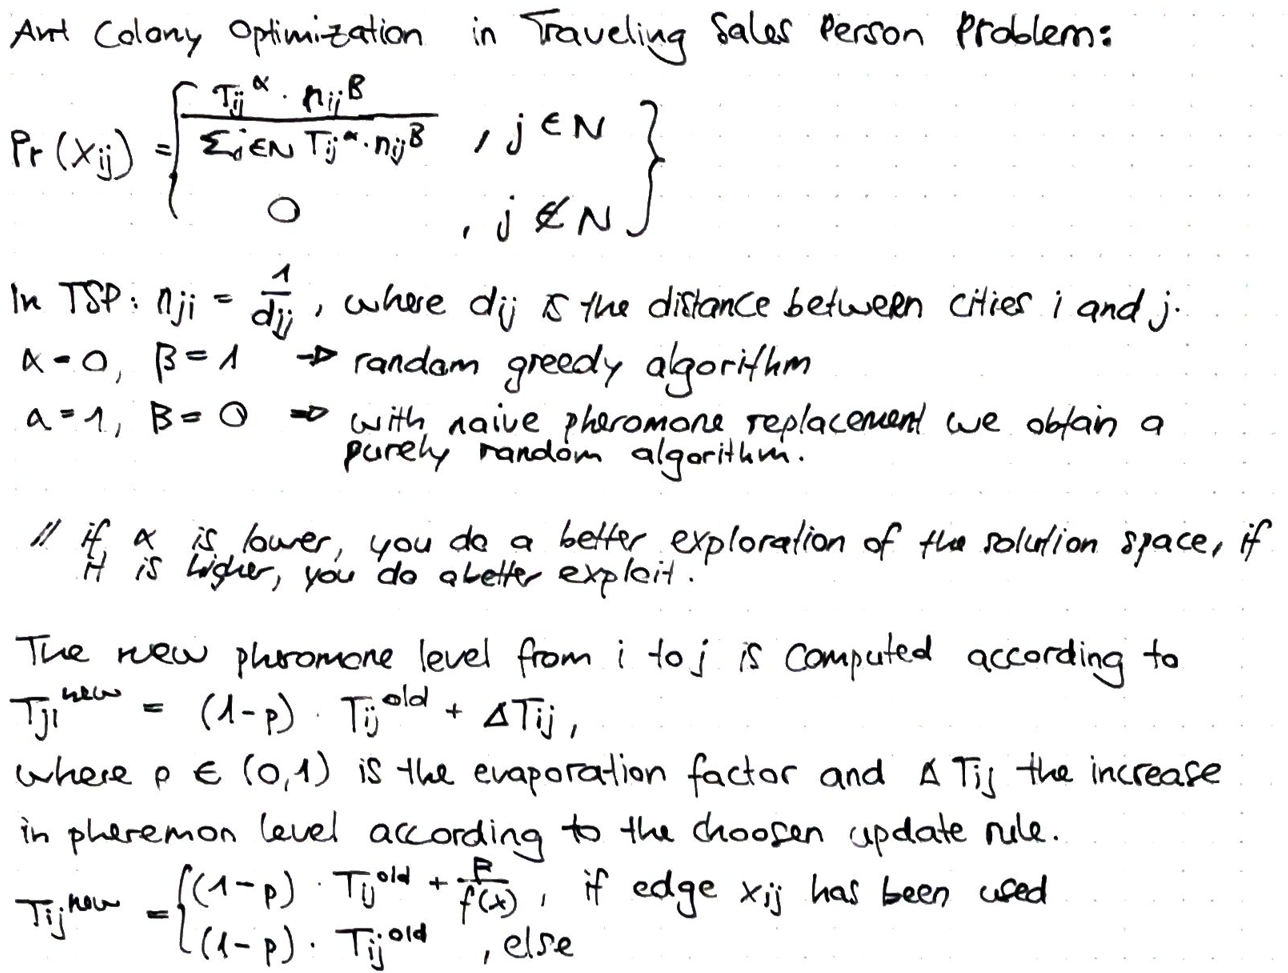
\includegraphics[width=0.9\textwidth]{figures/ants.png}
\caption{Ant Colony}
\end{figure}

\clearpage